\chapter{Анализ предметной области}
\label{cha:analysis}
\section{Компьютерное обучение иностранным языкам}

Для решения одной из поставленных задач необходимо определить обучающие методы, благодаря которым пользователь сможет эффективно усваивать знания. Наиболее часто в подобных приложениях можно встретить параллельные тексты и метод интервальных повторений, который чаще всего используется совместно с системой флэш-карточек.

\subsection{Параллельное чтение}

Параллельные тексты, вероятно, являются одним из самых древних методов обучения иностранным языкам. Данный метод заключается в представлении текста таким образом, что повествование идет сразу на двух языках: как правило, на одном обороте представлен исходный текст на изучаемом языке, а на другом~--- переведенный текст на родном языке.

Главное достоинство параллельного чтения~--- развитие <<чувства языка>>: анализируя и сравнивая два текста на разных языках, пользователь начинает лучше понимать структуру предложения, принципы его построения и те или иные языковые особенности.

Сложность в использовании этого метода состоит в том, что пользователю необходимо знать базовую грамматику и правила чтения. Кроме того, немаловажную роль играет качество перевода. Однако стоит отметить, что длительное использование параллельного чтения приводит к постепенному привыканию к различным лексическим и грамматическим конструкциям, что делает данный метод очень интересным и перспективным; также он отлично подходит для пополнения словарного запаса \cite{shepherd}.

\subsection{Метод интервальных повторений}

История появления данного метода началась в конце XIX века, когда немецкий психолог Герман Эббингауз построил «кривую забывания», отражающую то, как долго хранится в памяти однажды запомненная информация. Свои результаты он нанес на график и получил эту «кривую», показанную на рис.~\ref{fig:curve} (картинка взята отсюда \cite{picture}).

\begin{figure}
  \centering
  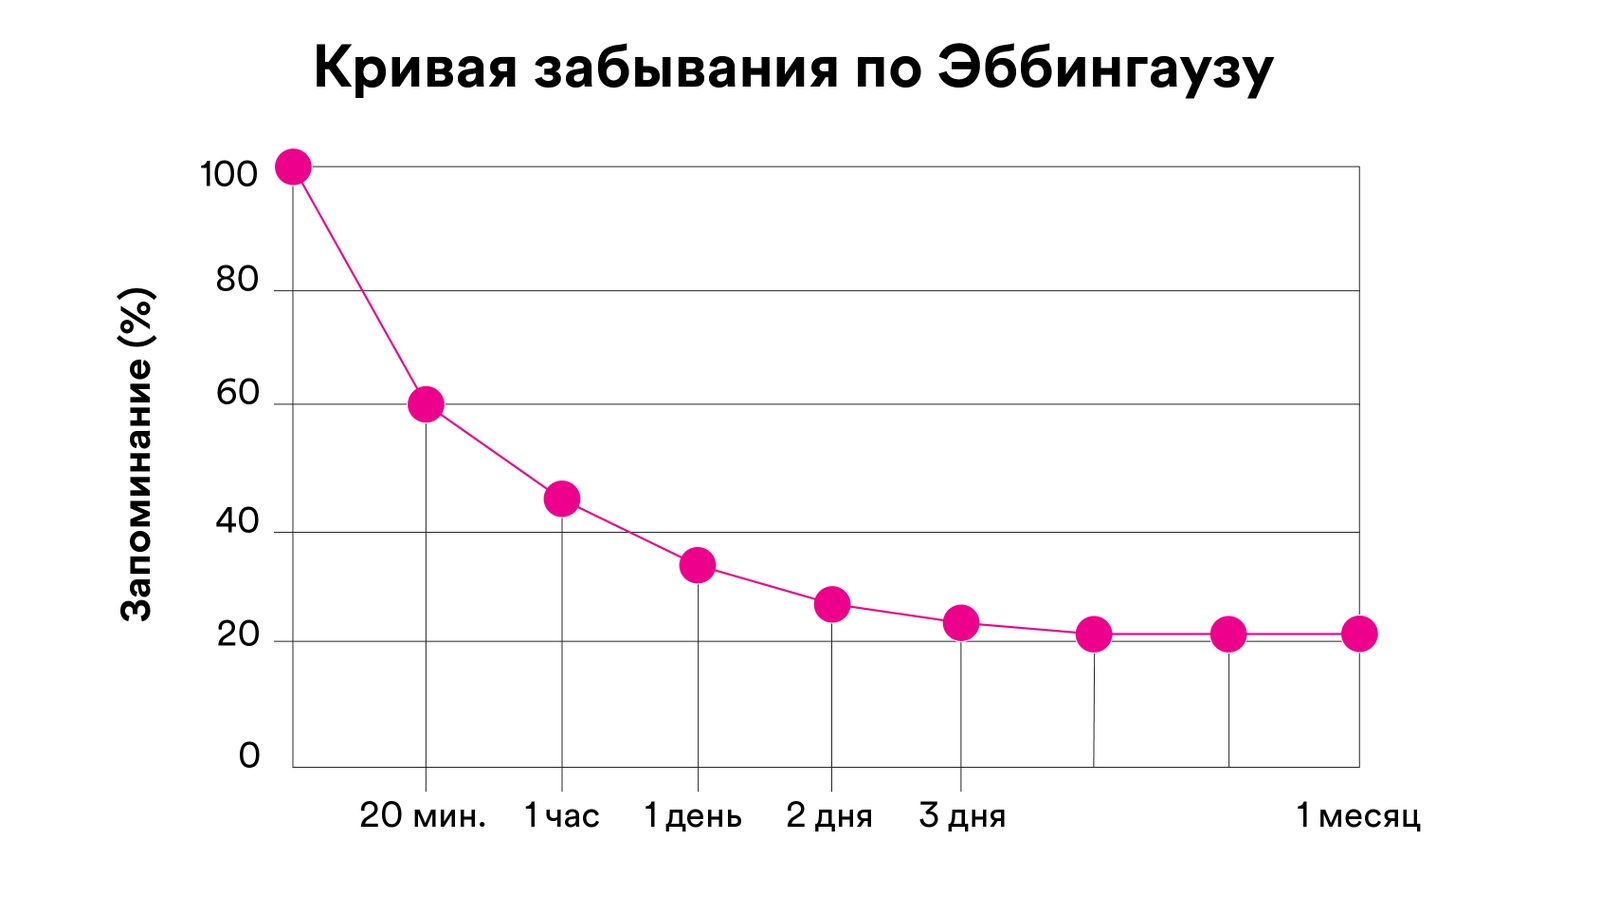
\includegraphics[width=\textwidth]{figures/curve}
  \caption{Кривая забывания}
  \label{fig:curve}
\end{figure}

Согласно его труду, если не пытаться осмысленно повторять однажды заученную информацию, то уже в течение первого часа забывается около 55\% всей информации; к концу дня это число становится равным около 36\%; далее процесс забывания идет медленно, и через неделю, равно как и через месяц, в памяти остается около 20\% от общего числа первоначально выученной информации \cite{ebbinghaus}.

В свою публикацию Эббингауз также включил уравнение аппроксимации этой кривой (\ref{F:F1}), где \textit{k} и \textit{c} — константы, полученные при определенных вычислениях (\textit{k} = 1.84, \textit{c} = 1.25), значение \textit{b} отражает «удержание» информации в процентах, тогда как \textit{t} равно времени в минутах.

\begin{equation}
b = 100 \times \frac{k}{{(\log_{10} t)}^c + k}
\label{F:F1}
\end{equation}

Впоследствии Эббингауз открыл \textit{закон накопления и распределения повторений}, окончательно сформулированный в 1895 году немецким психологом Адольфом Йостом. Согласно этому закону, при фиксированном количестве повторений распределенные во времени повторения более эффективны, чем одновременные.

Затем эта идея получила развитие в 1932 году, когда британский философ Алек Мейс разработал метод интервальных повторений \cite{mace}. Суть остается такой же: если осмысленно воспроизводить заученный материал через определенные, постоянно возрастающие интервалы времени, можно добиться более эффективных результатов и удержать выученную информацию на более длительные сроки.

В 1939 году было проведено исследование, в котором принимали участие более 3600 студентов, в ходе которого была доказана эффективность данного метода \cite{spitzer}. Несмотря на то, что эта техника подойдет для запоминания любой информации, наибольшее распространение она получила именно при изучении иностранных языков.

Как уже было упомянуто ранее, интервальные повторения часто используют совместно с системой флэш-карточек, также известной как система Лейтнера. Это простая реализация метода интервальных повторений, предложенная немецким журналистом и популяризатором науки Себастьяном Лейтнером в 1970-х годах \cite{leitner}. Она наглядно показана на рис.~\ref{fig:leitner}.

\begin{figure}
	\centering
	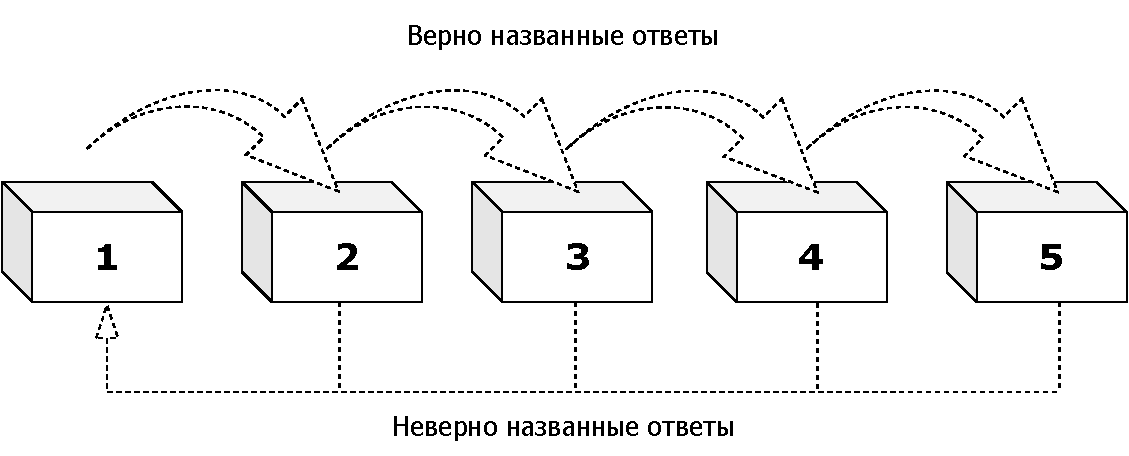
\includegraphics[keepaspectratio, scale=0.8]{figures/leitner}
	\caption{Система Лейтнера}
	\label{fig:leitner}
\end{figure}

Работает эта система следующим образом: в самом начале любое слово, представленное в виде карточки, всегда находится в первой коробке; если пользователь вспоминает его значение и отвечает правильно, то карточка перекладывается в следующую коробку, если отвечает неправильно — карточка возвращается назад в первую коробку, независимо от того, в какой коробке находилась на последней итерации. И каждое следующее слово повторяется через увеличивающийся интервал времени. Например, можно увеличивать время следующего повторения в три раза: в таком случае первое повторение наступит через день, второе~--- через 3 дня, третье~--- через 9 дней, четвертое~--- через 27 и т.~д.

\section{Обзор существующих приложений, предназначенных для обучения иностранным языкам}

В настоящее время существует достаточно обширное количество программных платформ для изучения иностранных языков. Стоит признать, что подавляющее большинство таких приложений преобладает на мобильном рынке, и чаще всего такие приложения являются либо платными, либо условно-бесплатными, причем условно-бесплатные решения сильно ограничены по своему функционалу и контентному содержимому. По этой причине мобильный сегмент рассматриваться не будет.

В рамках проведенного обзора были рассмотрены следующие наиболее популярные приложения, которые помогают в освоении иностранного языка:

\begin{itemize}
\item \textbf{Anki}~--- программа, предназначенная для облегчения запоминания слов, выражений и любой другой информации с помощью метода интервальных повторений;
\item \textbf{Duolingo}~--- бесплатный веб-сервис, который привлекает своим простым и понятным интерфейсом и игровым подходом к изучению иностранных языков.
\end{itemize}

\subsection{Anki}

Данная программа распространяется под свободной лицензией и доступна для использования на различных операционных системах: Microsoft Windows, macOS, Linux и FreeBSD. Существует веб-версия этого приложения с поддержкой хостинга колод и наличием разнообразных плагинов. Также авторами поддерживается мобильное приложение для iOS с закрытым исходным кодом.

Anki предоставляет пользователю следующий ряд интересных действий и возможностей:

\begin{itemize}
	\item создавать собственные карточки и настраивать их внешний вид различными способами: с помощью гипертекстовой разметки со стилями или продвинутыми средствами \LaTeX{}, а также оснащать их изображениями, звуками и мультимедийными файлами;
	\item настраивать алгоритмы обучения под собственные нужды;
	\item синхронизировать карточки между несколькими устройствами;
	\item просматривать подробную статистику в виде цифр и графиков.
\end{itemize}

Anki использует алгоритм, основанный на методе интервального повторения. Интерфейс десктопного приложения Anki представлен на рис.~\ref{fig:anki}. При нажатии кнопки <<Показать ответ>> необходимо указать то, насколько легко пользователю далось данное слово: <<не помню>>, <<в самый раз>>, <<очень легко>>. На основании статистики полученных ответов Anki определяет, какую карточку и когда нужно показывать для последующего повторения.

\begin{figure}[h]
	\centering
	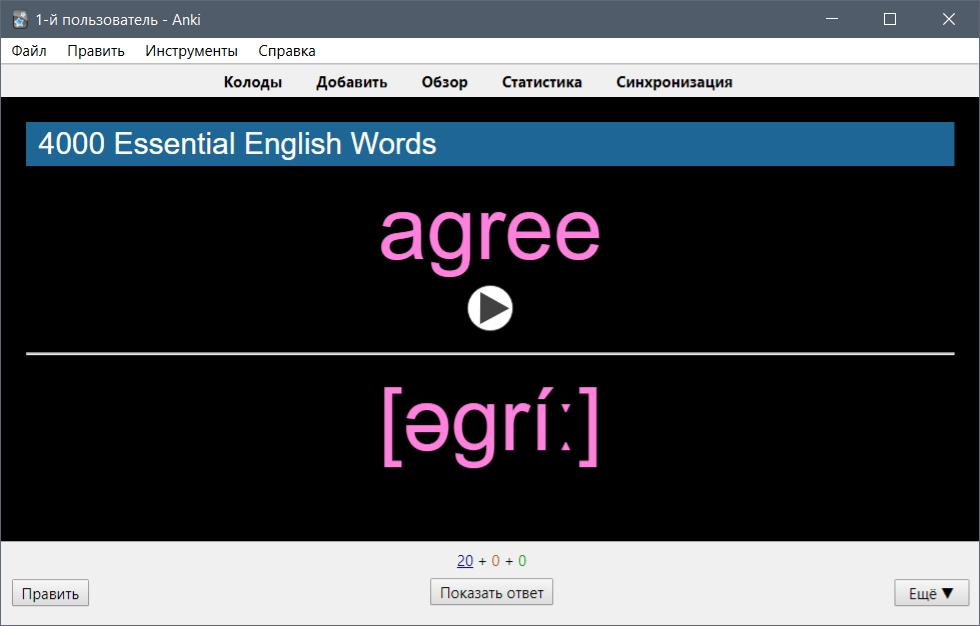
\includegraphics[keepaspectratio, scale=0.7]{figures/anki}
	\caption{Программный интерфейс десктопной версии Anki}
	\label{fig:anki}
\end{figure}

Можно практиковать как свои колоды карт, так и готовые колоды из Интернета. Более продвинутые колоды оснащены возможностью озвучивания слов и прочтения их транскрипций.

\subsection{Duolingo}

Duolingo является наиболее популярным веб-сервисом в международном сегменте. Платформа поддерживает обширный перечень языков и предлагает многочисленные вариации обучения: благодаря игровому дереву происходит продвижение по урокам, а в словарном разделе пользователи могут практиковать новые слова. Фрагмент игрового дерева представлен на рис.~\ref{fig:duo}.

\begin{figure}[h]
	\centering
	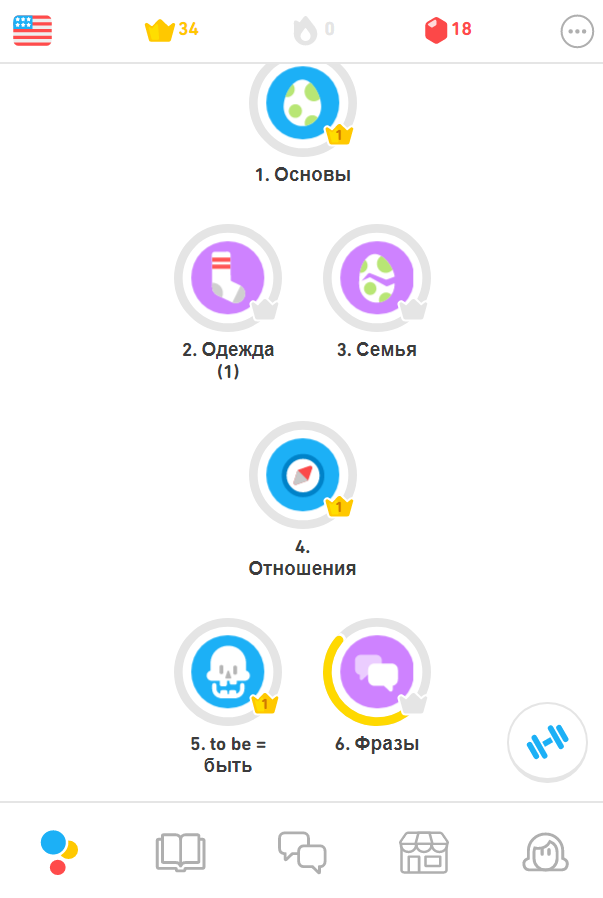
\includegraphics[width=0.6\textwidth, keepaspectratio]{figures/duo}
	\caption{Игровое дерево в Duolingo}
	\label{fig:duo}
\end{figure}

Для привлечения пользователей платформа имитирует структуру видеоигр: например, за счет системы вознаграждений пользователи могут получить внутреигровую валюту, которую можно потратить на бонусные уровни. Также существуют значки, которые представляют собой достижения и указывают на уровень квалификации пользователя.

В Duolingo также существуют системы форумов и т.~н. <<списки лидеров>>, которые позволяют повысить конкурентоспособность и отношения между пользователями, добавив учебному процессу больше веселья, что позволяет повысить мотивацию к обучению.

Главной особенностью Duolingo являются индивидуальные уроки: система запоминает и учитывает трудности, которые возникли у пользователя во время изучения языка, и использует эти данные для машинного обучения. Кроме того, по мере прохождения уроков пользователи параллельно помогают переводить сайты и различные документы.

Данная платформа доступна как в виде веб-приложения, так и в форме приложения под мобильные устройства на iOS и Android, однако далеко не все функции и возможности веб-приложения доступны в мобильной версии: к примеру, в ней отсутствует грамматическая справка, в которой приводится краткая сводка основных правил перед прохождением урока; также в мобильной версии нет возможности выбрать тренировку на время и общаться с другими пользователями на форуме.

\section{Вывод}

В данном разделе был проведен анализ предметной области, на основе которого были сделаны следующие выводы и наблюдения:

\begin{itemize}
	\item рассмотренные методики обучения имеют доказанную эффективность на основе ряда исследований и могут быть использованы для разрабатываемого приложения;
	\item геймификация процесса обучения и возможность пользовательского взаимодействия друг с другом~--- неотъемлемые черты подобных приложений для поддержания мотивации к обучению;
	\item возможным решением задачи обеспечения взаимодействия пользователя с разрабатываемым приложением является создание адаптивного веб-интерфейса, доступного под любые устройства через веб-браузер;
	\item одностраничные приложения выступают наиболее удачным решением для достижения интерактивного взаимодействия пользователя с веб-интерфейсом: мгновенная отрисовка данных и переключение между состояниями приложения благоприятно влияют на пользовательский опыт.
\end{itemize}

Проведенный обзор также показал распространенность использования веб-приложений для компьютерного обучения, что еще раз подчеркивает актуальность данной работы. Кроме того, ни одно из рассмотренных популярных приложений не сочетает в себе совместное использование метода параллельного чтения и системы интервальных повторений, что делает данную работу уникальной.

Таким образом, с учетом сделанных выводов становится возможным создание веб-приложения, в котором будут учтены наблюдения, подмеченные в данном разделе.

%%% Local Variables:
%%% mode: latex
%%% TeX-master: "rpz"
%%% End:
